\documentclass[12pt,a4paper,oneside]{report}

% --------------------------------------------------------------------------
% Packages and page layout
% --------------------------------------------------------------------------
\usepackage[T1]{fontenc}
\usepackage[utf8]{inputenc}
\usepackage{tgpagella}
\usepackage{newpxmath}
\usepackage{microtype}
\usepackage{csquotes}
\usepackage[english]{babel}
\usepackage[a4paper,top=1in,bottom=1in,left=1.25in,right=1in]{geometry}
\usepackage{setspace}
\usepackage{graphicx}
\usepackage{amsmath}
\usepackage{booktabs,tabularx,array,longtable}
\usepackage{enumitem}
\usepackage{caption}
\usepackage{chngcntr}
\usepackage{placeins}
\usepackage{float}
\usepackage{tocloft}
\usepackage{titlesec}
\usepackage{fancyhdr}
\usepackage[hidelinks]{hyperref}
\usepackage{bookmark}
\usepackage{tikz}
\usetikzlibrary{arrows.meta,positioning,shapes.geometric,fit}

\setstretch{1.25}
\setlength{\parindent}{1.25em}
\setlength{\parskip}{0.18em}
\setlist[itemize]{leftmargin=2.2em,itemsep=0.2em,topsep=0.3em}
\setlist[enumerate]{leftmargin=2.2em,itemsep=0.2em,topsep=0.3em}
\captionsetup{font=small,labelfont=bf,justification=centering,singlelinecheck=false}
\counterwithout{figure}{chapter}
\counterwithout{table}{chapter}
\emergencystretch=2em

\titleformat{\chapter}[display]
  {\normalfont\bfseries\centering}
  {\MakeUppercase{\chaptertitlename~\thechapter}}
  {0.45em}
  {\Large\bfseries\MakeUppercase}
\titleformat{name=\chapter,numberless}[display]
  {\normalfont\bfseries\centering}
  {}
  {0pt}
  {\Large\bfseries\MakeUppercase}
\titlespacing*{\chapter}{0pt}{-18pt}{24pt}
\titlespacing*{name=\chapter,numberless}{0pt}{-18pt}{24pt}
\titleformat{\section}{\normalfont\bfseries\large}{\thesection}{0.7em}{}
\titlespacing*{\section}{0pt}{1.2em}{0.35em}
\titleformat{\subsection}{\normalfont\bfseries\normalsize}{\thesubsection}{0.7em}{}

\pagestyle{fancy}
\fancyhf{}
\fancyfoot[C]{\thepage}
\renewcommand{\headrulewidth}{0pt}
\renewcommand{\footrulewidth}{0pt}
\fancypagestyle{plain}{%
  \fancyhf{}
  \fancyfoot[C]{\thepage}
  \renewcommand{\headrulewidth}{0pt}
  \renewcommand{\footrulewidth}{0pt}}

\hypersetup{
  pdftitle={MockMATE: An AI-Powered Interview Platform for Students},
  pdfauthor={Adarsh Bhaktha K, Vidhath N Shetty, Aboobacker Ruvais, Pavan Kumar}
}
\renewcommand{\contentsname}{CONTENTS}
\renewcommand{\listfigurename}{LIST OF FIGURES}
\renewcommand{\listtablename}{LIST OF TABLES}
\setcounter{tocdepth}{2}
\setcounter{secnumdepth}{2}
\renewcommand{\cftchapfont}{\bfseries}
\renewcommand{\cfttoctitlefont}{\hfill\Huge\bfseries}
\renewcommand{\cftaftertoctitle}{\hfill}
\renewcommand{\cftloftitlefont}{\hfill\Huge\bfseries}
\renewcommand{\cftafterloftitle}{\hfill}
\renewcommand{\cftlottitlefont}{\hfill\Huge\bfseries}
\renewcommand{\cftafterlottitle}{\hfill}

% Use the supplied college emblem if it is placed at this path.
\newcommand{\collegeemblem}[1]{%
  \IfFileExists{figures/emblem-000.png}
    {
\includegraphics[width=#1]{figures/emblem-000.png}}
    {\fbox{\parbox[c][#1][c]{#1}{\centering\small College\\Emblem}}}
}

\begin{document}
\hypersetup{pageanchor=false}

% --------------------------------------------------------------------------
% Title page
% --------------------------------------------------------------------------
\begin{titlepage}
\thispagestyle{empty}
\begin{center}
\vspace*{0.35cm}
{\bfseries\fontsize{16}{20}\selectfont
MOCKMATE: AN AI-POWERED\\[0.15em]
INTERVIEW PLATFORM FOR STUDENTS\par}

\vspace{0.75cm}
{\itshape Project Report (Phase I)\par}
\vspace{0.25cm}
{\itshape Submitted to the APJ Abdul Kalam Technological University\\
in partial fulfilment of the requirements for the award of the degree\par}
\vspace{0.45cm}
{\bfseries Bachelor of Technology\par}
\vspace{0.08cm}
in\par
\vspace{0.08cm}
{\bfseries Computer Science and Engineering\par}
\vspace{0.22cm}
by\par
\vspace{0.12cm}
{\bfseries ADARSH BHAKTHA K (KSD23CS010)\par}
{\bfseries VIDHATH N SHETTY (KSD23CS128)\par}
{\bfseries ABOOBACKER RUVAIS (KSD23CS009)\par}
{\bfseries PAVAN KUMAR (KSD23CS097)\par}

\vspace{0.55cm}
\collegeemblem{3.0cm}\par
\vfill
{\bfseries\small DEPARTMENT OF COMPUTER SCIENCE AND ENGINEERING\par}
\vspace{0.12cm}
{\bfseries\small LBS COLLEGE OF ENGINEERING, KASARAGOD\par}
\vspace{0.18cm}
{\bfseries November 2026\par}
\vspace*{0.25cm}
\end{center}
\end{titlepage}

\hypersetup{pageanchor=true}
\pagenumbering{roman}
\setcounter{page}{1}

% --------------------------------------------------------------------------
% Department vision and mission
% --------------------------------------------------------------------------
\clearpage
\thispagestyle{plain}
\begin{center}
{\bfseries\small LBS COLLEGE OF ENGINEERING, KASARAGOD\par}
{\small MULIYAR -- 671 542\par}
\vspace{0.45cm}
{\bfseries\large DEPARTMENT OF COMPUTER SCIENCE AND ENGINEERING\par}
\vspace{0.9cm}
{\bfseries\large Vision of Department\par}
\vspace{0.2cm}
\begin{minipage}{0.88\textwidth}\centering
To be a renowned centre for education, research, and innovation in the frontier areas of Computer Science and Engineering.
\end{minipage}
\end{center}
\vspace{0.85cm}
\begin{center}\textbf{\large Mission of Department}\end{center}
\vspace{0.2cm}
\begin{itemize}
\item Establish and maintain an operational environment to acquire, impart, create and apply knowledge in Computer Science and Engineering and interdisciplinary areas.
\item Serve as a resource centre for innovation in the design and development of hardware and software solutions.
\item Inculcate leadership qualities, professional ethics and a sense of social commitment.
\end{itemize}
\vfill
\clearpage

% --------------------------------------------------------------------------
% Certificate
% --------------------------------------------------------------------------
\thispagestyle{plain}
\begin{center}
{\bfseries\small DEPARTMENT OF COMPUTER SCIENCE AND ENGINEERING\par}
{\bfseries\small LBS COLLEGE OF ENGINEERING, KASARAGOD\par}
{\small MULIYAR -- 671 542\par}
{\small 2026--27\par}
\vspace{0.4cm}
\collegeemblem{2.0cm}\par
\vspace{0.2cm}
{\bfseries\Large CERTIFICATE\par}
\end{center}
\vspace{0.75cm}
This is to certify that the report entitled \emph{MockMATE: An AI-Powered Interview Platform for Students}, submitted by \textbf{Adarsh Bhaktha K (KSD23CS010), Vidhath N Shetty (KSD23CS128), Aboobacker Ruvais (KSD23CS009) and Pavan Kumar (KSD23CS097)} to the APJ Abdul Kalam Technological University in partial fulfilment of the requirements for the B.Tech. degree in Computer Science and Engineering, is a bona fide record of the Phase I project work carried out by them under our guidance and supervision. This report has not previously been submitted to any other university or institute for any purpose.

\vspace{1.35cm}
\noindent
\begin{minipage}[t]{0.43\textwidth}
\vspace{0pt}
\raggedright
\textbf{Prof. Reema K V}\\
(Project Guide)\\
Associate Professor\\
Department of CSE\\
LBS College of Engineering
\end{minipage}
\hfill
\begin{minipage}[t]{0.43\textwidth}
\vspace{0pt}
\raggedright
\textbf{Prof. Jayalekshmi S}\\
(Project Coordinator)\\
Associate Professor\\
Department of CSE\\
LBS College of Engineering
\end{minipage}

\vspace{1.45cm}
\begin{center}
\textbf{Dr. Jayalekshmi S}\\
Professor and Head\\
Department of CSE\\
LBS College of Engineering\\
Kasaragod
\end{center}
\vfill
\clearpage

% --------------------------------------------------------------------------
% Declaration
% --------------------------------------------------------------------------
\chapter*{DECLARATION}
\thispagestyle{plain}
\vspace{0.35cm}
We hereby declare that the Phase I project report entitled \emph{MockMATE: An AI-Powered Interview Platform for Students}, submitted in partial fulfilment of the requirements for the award of the degree of Bachelor of Technology in Computer Science and Engineering under the APJ Abdul Kalam Technological University, Kerala, is a bona fide record of the work carried out by us under the supervision of Prof. Reema K V.

This submission represents our work and ideas in our own words. Wherever the ideas or words of others have been included, the original sources have been acknowledged through appropriate references.

We further declare that we have adhered to the principles of academic honesty and integrity and have not knowingly misrepresented or fabricated any data, idea, fact or source in this report. This report has not previously formed the basis for the award of any degree, diploma or similar title from any other university or institution.

\vspace{1.0cm}
\noindent
\begin{minipage}[t]{0.5\textwidth}
Place: Kasaragod\\
Date: 01-11-2026
\end{minipage}%
\begin{minipage}[t]{0.5\textwidth}
\raggedleft
\textbf{PROJECT TEAM}\\
Adarsh Bhaktha K\\
Vidhath N Shetty\\
Aboobacker Ruvais\\
Pavan Kumar
\end{minipage}
\clearpage

% --------------------------------------------------------------------------
% Acknowledgement
% --------------------------------------------------------------------------
\chapter*{ACKNOWLEDGEMENT}
\addcontentsline{toc}{chapter}{ACKNOWLEDGEMENT}
\thispagestyle{plain}
We express our sincere gratitude to everyone who supported us during the preparation of this Phase I project report.

We thank Dr. Jayalekshmi S, Professor and Head of the Department of Computer Science and Engineering, LBS College of Engineering, Kasaragod, for providing the facilities and academic support required for the project.

We express our gratitude to Prof. Jayalekshmi S, Project Coordinator, for the guidance and cooperation provided during the project phase. We are especially grateful to our project guide, Prof. Reema K V, Associate Professor, Department of Computer Science and Engineering, for her guidance, suggestions and constructive feedback throughout the planning and preparation of this work.

We also acknowledge the support of the Department of Computer Science and Engineering, our faculty members, classmates, friends and family, whose assistance contributed to the completion of this report.

\vspace{1cm}
\begin{flushright}
\textbf{PROJECT TEAM}
\end{flushright}
\clearpage

% --------------------------------------------------------------------------
% Abstract
% --------------------------------------------------------------------------
\chapter*{ABSTRACT}
\addcontentsline{toc}{chapter}{ABSTRACT}
\thispagestyle{plain}
Technical interviews are an important part of recruitment for software development and other computing-related roles. However, students and fresh graduates may have limited opportunities to practise in a realistic interview environment and to receive structured feedback on their performance. Conventional mock interviews generally require another person to conduct and evaluate the session, which can make repeated practice difficult to arrange.

MockMATE is proposed as an AI-powered interview practice platform intended primarily for students. The initial project scope focuses on Python technical interviews. It is designed to allow a candidate to participate through chat, audio and camera-based inputs. The platform aims to evaluate technical responses and provide additional feedback on communication and selected observable interview behaviours. At the end of a session, it is intended to generate a personalised report that identifies strengths and areas requiring improvement.

The Phase I work studies existing AI-based mock interview systems, multimodal candidate assessment, natural language processing, emotion recognition and adaptive question generation. The literature review is used to identify limitations in existing approaches and to establish the motivation and objectives of the proposed system. The report also presents the proposed system design, its major modules, preliminary technology considerations and the expected outcomes. The implementation details and measured performance are outside the scope of this Phase I report and will be addressed during subsequent development and evaluation.
\clearpage

% --------------------------------------------------------------------------
% Contents
% --------------------------------------------------------------------------
\tableofcontents
\clearpage
\addcontentsline{toc}{chapter}{LIST OF FIGURES}
\listoffigures
\clearpage
\addcontentsline{toc}{chapter}{LIST OF TABLES}
\listoftables
\clearpage

\pagenumbering{arabic}
\setcounter{page}{1}

% ==========================================================================
% Chapter 1
% ==========================================================================
\chapter{Introduction}

\section{Background}
Technical interviews are widely used by organisations to assess the suitability of candidates for software development and other technical positions. These interviews may evaluate programming knowledge, problem-solving ability, communication skills and the ability to explain technical decisions. For students and fresh graduates, performing well in an interview requires more than familiarity with a programming language. Candidates must also understand questions, organise their thoughts, explain solutions clearly and respond appropriately to follow-up questions.

Many students have limited access to realistic interview practice. Practice opportunities may depend on the availability of peers, mentors, faculty members or professional interviewers. Even when practice sessions are available, feedback may be informal or may not cover all relevant aspects of performance. As a result, candidates may find it difficult to identify recurring weaknesses and measure their improvement over multiple sessions.

Recent developments in artificial intelligence have created opportunities to automate parts of the interview-practice process. Natural language processing can be used to interpret written responses, speech recognition can convert spoken answers into text, and language models can support question generation and feedback generation. Audio and video processing techniques can provide additional information about a candidate's delivery and visible interview behaviour.

The project \emph{MockMATE: An AI-Powered Interview Platform for Students} proposes to bring these capabilities together in an accessible interview-practice platform. The initial version is intended to focus on Python technical interviews and support chat, audio and camera-based responses.

\section{Motivation}
The project is motivated by the need for a convenient and repeatable environment in which students can practise technical interviews. A candidate should be able to attempt an interview without having to arrange a human interviewer for every practice session. The system should also provide feedback that helps the candidate understand what was done well and what needs further attention.

The main motivations are:
\begin{itemize}
    \item To make technical interview practice more accessible to students and fresh graduates.
    \item To provide a low-pressure environment in which candidates can practise repeatedly.
    \item To reduce dependence on the availability of a human interviewer for routine practice.
    \item To assess technical responses and provide structured feedback.
    \item To include communication and observable interview behaviour as additional areas of feedback.
    \item To help candidates identify strengths and weaknesses through a session-based report.
\end{itemize}

\section{Problem Statement}
Many students and fresh graduates have limited opportunities to practise technical interviews in a realistic setting. They may find it difficult to evaluate the correctness and clarity of their technical answers, communication and confidence without detailed feedback. Traditional mock interviews depend on the availability of another person and may not support frequent, individual practice. Existing automated approaches may concentrate on only one aspect, such as question generation, speech analysis or emotion recognition.

Therefore, an accessible AI-assisted platform is proposed to support technical interview practice through multiple response modes and provide personalised feedback on technical answers, communication and selected observable interview behaviours.

\section{Aim}
The aim of the project is to design and develop an AI-powered mock interview platform that enables students to practise technical interviews and receive personalised feedback on their responses and interview performance.

\section{Objectives}
The objectives of MockMATE are:
\begin{enumerate}
    \item To develop an AI-powered interview practice platform primarily intended for students.
    \item To begin with Python-specific technical interview questions.
    \item To allow candidates to respond through text chat, audio and camera-based inputs.
    \item To analyse the technical content and relevance of candidate responses.
    \item To examine selected communication characteristics and observable interview behaviour.
    \item To generate personalised feedback highlighting strengths and areas for improvement.
    \item To design the platform so that it can be extended to other programming languages, technical domains, adaptive questions and resume-based personalisation.
\end{enumerate}

\section{Scope of the Project}
The initial scope is limited to a student-oriented mock interview platform with Python as its first technical domain. A candidate should be able to participate in an interview session using supported input modes and receive a summary of performance after the session.

The proposed system considers three response modes:
\begin{itemize}
    \item \textbf{Text mode:} the candidate enters answers through a chat interface.
    \item \textbf{Audio mode:} the candidate gives spoken answers, which can be transcribed for further analysis.
    \item \textbf{Camera-based mode:} the candidate participates with a camera enabled so that selected observable visual information can be considered.
\end{itemize}

The project is intended for learning and self-improvement. It is not proposed as a replacement for professional recruitment decisions. In particular, automated estimates of confidence, emotion or visible behaviour should be treated cautiously and should not be interpreted as definitive measures of a person's ability or personality.

\section{Organisation of the Report}
This report is organised into five chapters. Chapter 1 introduces the project, its motivation, problem statement, aim, objectives and scope. Chapter 2 reviews related research and identifies the gaps that motivate MockMATE. Chapter 3 presents the proposed system design and its overall workflow. Chapter 4 describes the major modules and preliminary software requirements. Chapter 5 concludes the Phase I work and outlines the proposed future activities.

% ==========================================================================
% Chapter 2
% ==========================================================================
\chapter{Literature Review}

\section{Introduction}
Artificial intelligence has been increasingly applied to interview simulation, candidate assessment and communication analysis. Existing research explores different parts of this problem, including automated question generation, speech processing, emotion recognition, multimodal assessment and conversational agents. Some systems focus on helping candidates practise, while others are designed primarily for recruitment and candidate screening.

The following review is based on the studies identified during the project literature survey. The studies are discussed in terms of their approach, contributions and limitations relevant to the proposed MockMATE platform.

\section{Study of Existing Works}

\subsection{AI Mock Interview System}
The work titled \emph{AI Mock Interview System} by Madhura Abhishek and Meenakshi Sheik describes a system that generates interview questions, records candidate answers, analyses responses and provides feedback. The approach aims to make interview practice convenient and reduce the need for a human interviewer in every session. Such a system can support repeated practice and quick feedback. However, automated assessment may not capture every aspect of human communication, and the usefulness of the feedback depends on the quality of the underlying analysis.

\subsection{Rider-AI Powered Mock Interview System with Real-Time Voice and Emotion Analysis}
Soni Khapekar et al. present a mock interview approach that combines interview question generation with voice and emotion analysis. The integration of voice-related information and emotion analysis provides a more interactive practice environment than a text-only system. However, emotion detection can be inaccurate, and recording conditions such as background noise and audio quality may affect the analysis.

\subsection{FairHire: AI-Driven Resume Profiling and Technical Interview Automation}
Akshay Baby et al. describe FairHire, which extracts skills from resumes, builds candidate profiles and generates technical interview questions. Linking resume analysis with question generation can make an interview more relevant to a candidate's stated experience. The approach can also reduce manual effort in initial screening. Its effectiveness depends on the quality of the candidate's resume data, and accurately interpreting open-ended responses remains a challenge.

\subsection{AI Based Mock Interview System Using NLP}
K. Senthilkumar et al. (2025) describe an AI-based mock interview system using speech-to-text, natural language processing, reinforcement learning, OpenCV, MediaPipe and text-to-speech. The approach considers technical, communication and behavioural aspects of an interview. Its use of several modalities and processing components offers a broad assessment pipeline. At the same time, noise and lighting conditions can affect input quality, while the combination of multiple technologies increases system complexity.

\subsection{MAG-BERT-ARL for Fair Automated Video Interview Assessment}
Bimasena Putra et al. (2024) investigate a multimodal approach for automated video interview assessment using BERT, audio and visual information, multimodal adaptation and adversarial learning. The work is relevant because it considers information from multiple input types and includes fairness as part of the assessment problem. However, such models can be computationally complex and require suitable training data. These requirements may make direct deployment in a lightweight student practice platform difficult.

\subsection{Candidate Evaluation with Multimodal Data-Driven for Recruitment}
Xing Wu et al. (2024) describe a recruitment-oriented candidate evaluation approach that uses graph-based methods, including GNN/GAT and DP-GNN, to process text, audio and image information. Combining several information sources can support a broader candidate evaluation process. The approach depends on high-quality data, and personality-related predictions may be inaccurate. Its main focus is recruitment evaluation rather than adaptive technical interview practice.

\subsection{Conversate: Supporting Reflective Learning in Interview Practice Through Interactive Simulation and Dialogic Feedback}
Taufiq Daryanto et al. (2025) present Conversate, an interactive interview-practice approach that uses Whisper for speech-to-text, GPT-3.5-Turbo for interview simulation, GPT-4 for feedback, and MongoDB and Firebase for storage. The system supports interactive dialogue and adaptive follow-up questions. Its reflective feedback model is relevant to a student-focused practice platform. However, the quality and consistency of the generated questions and feedback depend on the AI models and their configuration.

\subsection{MOCKLLM: A Multi-Agent Behavior Collaboration Framework for Online Job Seeking and Recruiting}
Hongda Sun et al. (2025) propose MOCKLLM, a multi-agent framework for online job seeking and recruitment. The described approach uses Nanbeige-16B-Chat, multi-agent role-play, vLLM, reflection memory and a handshake protocol. Multi-agent interaction can support multi-turn practice and reflection across interactions. The framework is more complex and resource-intensive than a single-agent approach, which is an important consideration for the scope of MockMATE.

\subsection{Single- vs. Dual-Prompt Dialogue Generation with LLMs for Job Interviews}
Joachim De Baer et al. (2025) study dialogue generation for job interviews using GPT-4o and Llama 3.3 70B, with interviewer and candidate role agents and a Llama-based judging component. Role-based prompting can produce more structured and human-like interview dialogue. However, using dual prompts increases token consumption and can raise API or computational costs.

\subsection{Candidate Evaluation with Multimodal Data-Driven for Recruitment (ICPR 2024)}
The literature survey also lists a work by X. Wu et al. under the title \emph{Candidate Evaluation with Multimodal Data-Driven for Recruitment (ICPR 2024)}. It describes the combination of graph neural networks with text, audio and image processing for candidate assessment. The approach supports multimodal evaluation, but it requires quality data and does not specifically focus on adaptive technical interview questions. This entry is retained as a separate item because it appears separately in the supplied survey material; its bibliographic relationship to the Xing Wu et al. entry above should be verified before final submission.

\subsection{Multi-Label Multimodal Emotion Recognition with Transformer-Based Fusion}
Y. Wang et al. (2023) examine multimodal emotion recognition using video, audio and text with transformer-based fusion. The approach aims to recognise multiple emotions and relationships between different input modalities. Although relevant to the visual and audio analysis aspects of MockMATE, the method is computationally demanding and focuses primarily on emotion recognition rather than interview practice as a whole.

\subsection{Experience-Aware Question Generation: A Personalized Approach}
Mallikarjuna G. D. et al. (2025) describe an experience-aware question generation approach that analyses resume information and experience using natural language processing and Bloom's Taxonomy to determine question difficulty. This can help personalise questions according to a candidate's experience level. However, the method depends on the completeness and accuracy of resume information, question quality can vary, and the described approach does not include video analysis.

\section{Literature Comparison}
Table~\ref{tab:literature-comparison} summarises the research works included in the supplied literature survey.

\begingroup
\small
\sloppy
\setlength{\tabcolsep}{4pt}
\renewcommand{\arraystretch}{1.35}
\begin{longtable}{|>{\centering\arraybackslash}p{0.55cm}|>{\raggedright\arraybackslash}p{3.0cm}|>{\raggedright\arraybackslash}p{2.2cm}|>{\raggedright\arraybackslash}p{4.0cm}|>{\raggedright\arraybackslash}p{3.6cm}|}
\hline
\textbf{No.} & \textbf{Work / Author} & \textbf{Focus} & \textbf{Method / Contribution} & \textbf{Limitation} \\
\hline
\endfirsthead
\hline
\textbf{No.} & \textbf{Work / Author} & \textbf{Focus} & \textbf{Method / Contribution} & \textbf{Limitation} \\
\hline
\endhead
1 & AI Mock Interview System; Madhura Abhishek and Meenakshi Sheik & Interview practice & Question generation, answer recording, response analysis and feedback. & May not capture all human communication details. \\
\hline
2 & Rider-AI Powered Mock Interview System; Soni Khapekar et al. & Voice and emotion analysis & Simulated interview with question generation and voice/emotion analysis. & Emotion detection and recording quality may affect results. \\
\hline
3 & FairHire; Akshay Baby et al. & Resume-based technical interviews & Resume skill extraction, candidate profiling and technical question generation. & Depends on resume quality and response interpretation. \\
\hline
4 & AI Based Mock Interview System Using NLP; K. Senthilkumar et al. (2025) & Multimodal mock interviews & STT, NLP, reinforcement learning, OpenCV, MediaPipe and TTS. & Input conditions and system complexity. \\
\hline
5 & MAG-BERT-ARL; Bimasena Putra et al. (2024) & Video interview assessment & BERT-based multimodal assessment with audio and visual information. & High data and computational requirements. \\
\hline
6 & Candidate Evaluation with Multimodal Data-Driven for Recruitment; Xing Wu et al. (2024) & Recruitment assessment & Graph-based processing of text, audio and image information. & Not focused on adaptive student practice. \\
\hline
7 & Conversate; Taufiq Daryanto et al. (2025) & Reflective interview practice & Whisper, GPT-based simulation and feedback, and adaptive follow-up questions. & Output quality depends on AI model behaviour. \\
\hline
8 & MOCKLLM; Hongda Sun et al. (2025) & Multi-agent recruitment and practice & Multi-agent role-play with reflection memory. & Greater system and resource complexity. \\
\hline
9 & Single- vs. Dual-Prompt Dialogue Generation; Joachim De Baer et al. (2025) & LLM interview dialogue & Interviewer/candidate role agents and model-based judging. & Dual prompting increases token and API costs. \\
\hline
10 & Candidate Evaluation with Multimodal Data-Driven for Recruitment (ICPR 2024); X. Wu et al. & Multimodal recruitment evaluation & Graph neural networks combined with text, audio and image processing. & Requires quality data; not focused on adaptive technical questions. \\
\hline
11 & Multi-Label Multimodal Emotion Recognition; Y. Wang et al. (2023) & Emotion recognition & Transformer-based fusion of video, audio and text. & Computationally demanding; not an interview-practice system. \\
\hline
12 & Experience-Aware Question Generation; Mallikarjuna G. D. et al. (2025) & Personalised questions & Resume and experience analysis with NLP and Bloom's Taxonomy. & Depends on resume quality; no video analysis. \\
\hline
\caption{Comparison of the works included in the MockMATE literature survey.}
\label{tab:literature-comparison}
\end{longtable}
\endgroup

\section{Research Gap}
The reviewed works demonstrate that AI can support interview simulation, question generation, speech processing, multimodal analysis and automated feedback. However, the supplied survey indicates several gaps relevant to the proposed project:

\begin{itemize}
    \item \textbf{Limited depth of feedback:} Some systems provide interview simulation but may offer limited guidance on how a candidate can improve.
    \item \textbf{Fragmented assessment:} Some approaches analyse voice or emotion without fully evaluating the technical content of answers.
    \item \textbf{Limited adaptation:} Resume-based question generation may not necessarily adapt subsequent questions according to the candidate's actual responses.
    \item \textbf{Different target users:} Several multimodal systems are designed for recruitment or candidate screening rather than repeated practice by students.
    \item \textbf{Reliability of generated feedback:} AI-generated questions and feedback may be inaccurate or inconsistent.
    \item \textbf{Need for an integrated practice environment:} Students need a single platform that combines technical practice, communication feedback and selected observable interview behaviour.
\end{itemize}

\section{Proposed Approach}
MockMATE is proposed as a student-oriented interview practice platform that brings together technical question-and-answer practice with feedback from multiple input modes. The initial scope is Python technical interviews. The proposed system aims to analyse the candidate's answer, use audio or camera input where enabled, and present a consolidated feedback report. The project will prioritise understandable feedback and a practical student workflow rather than attempting to make automated hiring decisions.

% ==========================================================================
% Chapter 3
% ==========================================================================
\chapter{Proposed System Design}

\section{Overview}
MockMATE is planned as an AI-assisted platform through which a student can participate in a simulated technical interview. The system begins with the selection or creation of an interview session. It then presents questions, accepts the candidate's responses through the selected input mode and processes the collected information. After the session, the system is intended to generate a feedback report.

The proposed design separates the user interface, interview management, input processing, AI-based analysis and report generation. This modular structure allows individual components to be developed and evaluated independently.

\section{Overall Workflow}
The proposed workflow consists of the following stages:

\begin{enumerate}
    \item \textbf{User access:} The candidate opens the platform and enters the interview-practice workflow.
    \item \textbf{Interview setup:} The candidate selects the initial Python interview scope and the available response mode.
    \item \textbf{Question presentation:} The system presents a technical interview question.
    \item \textbf{Response collection:} The candidate submits a text answer or responds through audio or camera-enabled input.
    \item \textbf{Input processing:} The submitted response is prepared for analysis. Audio may be transcribed, while camera-based input may be processed for selected visual features.
    \item \textbf{Answer evaluation:} The system analyses the technical relevance and quality of the response.
    \item \textbf{Performance analysis:} Selected communication characteristics and observable interview behaviour are considered where the relevant input is available.
    \item \textbf{Feedback generation:} The system prepares a session report containing strengths and areas for improvement.
\end{enumerate}

\section{Proposed System Architecture}
Figure~\ref{fig:architecture} presents a high-level view of the proposed MockMATE architecture. It is a design-level representation for Phase I; the final implementation architecture may change after technology selection and development.

\begin{figure}[H]
\centering
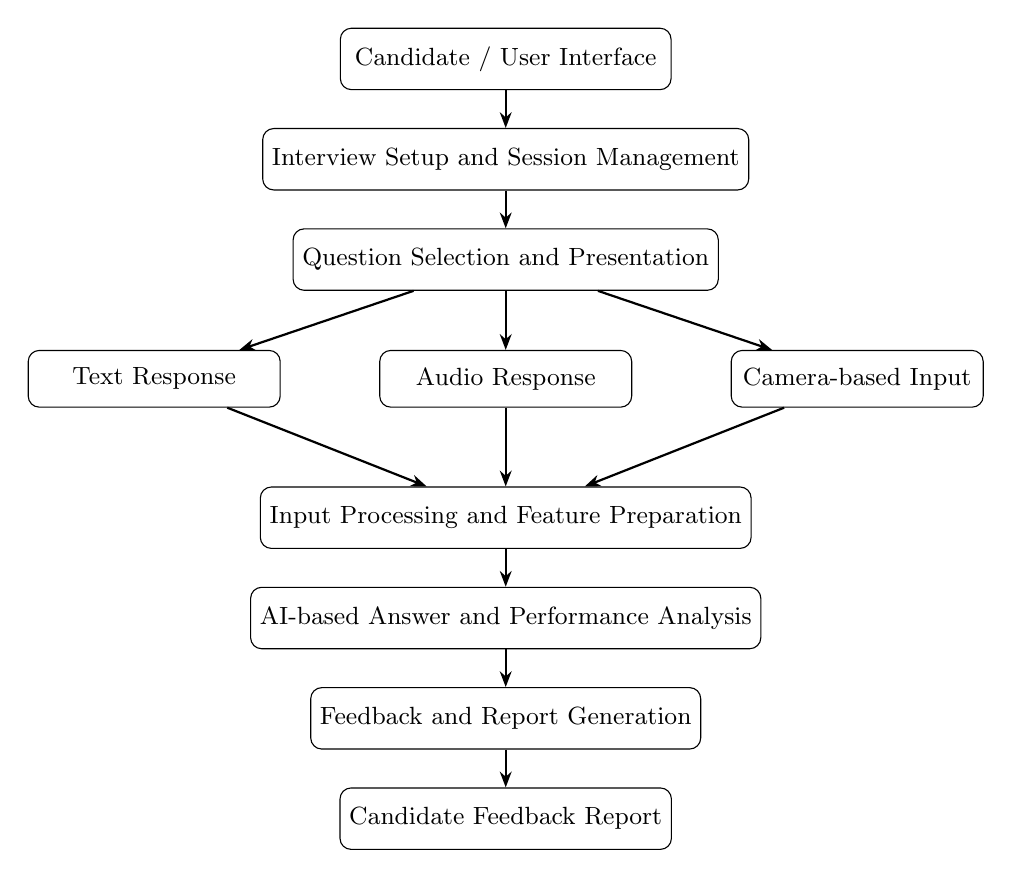
\begin{tikzpicture}[
    node distance=0.48cm and 0.8cm,
    block/.style={draw,rounded corners,align=center,minimum width=4.2cm,minimum height=0.78cm,font=\small},
    smallblock/.style={draw,rounded corners,align=center,minimum width=3.2cm,minimum height=0.72cm,font=\small},
    arrow/.style={-{Stealth[length=2mm]},thick}
]
\node[block] (user) {Candidate / User Interface};
\node[block,below=of user] (setup) {Interview Setup and Session Management};
\node[block,below=of setup] (questions) {Question Selection and Presentation};
\node[smallblock,below left=0.75cm and 0.15cm of questions] (text) {Text Response};
\node[smallblock,below=0.75cm of questions] (audio) {Audio Response};
\node[smallblock,below right=0.75cm and 0.15cm of questions] (video) {Camera-based Input};
\node[block,below=1.0cm of audio] (processing) {Input Processing and Feature Preparation};
\node[block,below=of processing] (analysis) {AI-based Answer and Performance Analysis};
\node[block,below=of analysis] (feedback) {Feedback and Report Generation};
\node[block,below=of feedback] (report) {Candidate Feedback Report};

\draw[arrow] (user) -- (setup);
\draw[arrow] (setup) -- (questions);
\draw[arrow] (questions) -- (text);
\draw[arrow] (questions) -- (audio);
\draw[arrow] (questions) -- (video);
\draw[arrow] (text) -- (processing);
\draw[arrow] (audio) -- (processing);
\draw[arrow] (video) -- (processing);
\draw[arrow] (processing) -- (analysis);
\draw[arrow] (analysis) -- (feedback);
\draw[arrow] (feedback) -- (report);
\end{tikzpicture}
\caption{High-level proposed architecture of MockMATE.}
\label{fig:architecture}
\end{figure}

\section{Description of Architecture Components}

\subsection{Candidate Interface}
The candidate interface is the entry point of the platform. It is intended to provide access to interview setup, question presentation, response submission and the final feedback report. The interface should make the practice process straightforward and should clearly indicate which input mode is active.

\subsection{Interview Session Management}
This component manages the sequence and state of an interview session. It coordinates question presentation and response collection. It should maintain the association between each question and the candidate's corresponding answer so that the responses can be evaluated in context.

\subsection{Question Selection and Presentation}
The question component supplies technical questions for the interview. The initial scope is Python. Questions should be presented in a clear sequence and should be suitable for the intended student-level practice. Adaptive follow-up questions and resume-based personalisation are considered possible extensions rather than confirmed features of the Phase I design.

\subsection{Input Processing}
The input-processing component prepares candidate responses for analysis. Text responses can be passed directly to language-processing components. Audio responses may require speech-to-text conversion. Camera-based input may require visual processing to obtain selected observable features. The exact processing methods and models will be finalised during implementation.

\subsection{AI-based Analysis}
The analysis component is intended to examine the technical content of the candidate's answer. Depending on the available input, it may also analyse communication characteristics and selected observable interview behaviours. The design separates technical answer evaluation from audio- or video-derived observations so that the limitations of each analysis can be communicated clearly.

\subsection{Feedback and Report Generation}
The final component combines the analysis results into a structured report. The report is intended to highlight areas in which the candidate performed well and areas that need improvement. Feedback should be specific enough to guide further practice and should avoid presenting uncertain behavioural estimates as objective facts.

\section{Data Flow}
The proposed data flow is as follows:
\begin{enumerate}
    \item The candidate starts an interview session.
    \item The system selects and displays a question.
    \item The candidate submits a response through text, audio or camera-enabled interaction.
    \item The response is stored or passed to the relevant processing component for the current session.
    \item The system prepares the response for technical and, where applicable, communication analysis.
    \item The analysis results are combined into a feedback summary.
    \item The candidate views the final report and uses it to guide subsequent practice.
\end{enumerate}

\section{Design Considerations}
The following considerations will guide the implementation:
\begin{itemize}
    \item \textbf{Usability:} The interview workflow should be understandable to students with different levels of technical experience.
    \item \textbf{Modularity:} Question management, input processing, analysis and reporting should be separable components.
    \item \textbf{Input flexibility:} The design should support text, audio and camera-based responses within the stated project scope.
    \item \textbf{Feedback clarity:} Reports should explain strengths and weaknesses in a way that candidates can act upon.
    \item \textbf{Privacy:} Audio and video data require careful handling, clear user consent and appropriate access controls.
    \item \textbf{Responsible assessment:} Observable behaviour or emotion-related outputs should be treated as uncertain signals and should not be used as definitive judgments about a candidate.
\end{itemize}

% ==========================================================================
% Chapter 4
% ==========================================================================
\chapter{Modules and Tools}

\section{Module Description}
The proposed MockMATE system is divided into five major modules. These modules describe the planned functional responsibilities of the Phase I design. Their final implementation details will be determined during the development phase.

\subsection{User Interface and Interview Management}
This module provides the candidate-facing interface and controls the interview session.

\textbf{Main responsibilities:}
\begin{itemize}
    \item Provide an interface to start and manage an interview session.
    \item Present questions in a readable and organised manner.
    \item Allow the candidate to select an available response mode.
    \item Maintain the sequence of questions and corresponding responses.
    \item Provide access to the generated feedback report.
\end{itemize}

\textbf{Expected outcome:} A consistent interface through which students can complete a mock interview.

\subsection{Question Management}
This module is responsible for selecting and presenting interview questions. The initial question domain is Python technical interviews.

\textbf{Main responsibilities:}
\begin{itemize}
    \item Organise questions according to the initial technical domain.
    \item Present questions during the interview session.
    \item Associate each response with its corresponding question.
    \item Provide a foundation for future support for additional domains and difficulty levels.
\end{itemize}

\textbf{Expected outcome:} An organised question flow suitable for student-level Python interview practice.

\subsection{Multimodal Response Collection and Processing}
This module collects candidate responses through the supported interaction modes and prepares them for analysis.

\textbf{Main responsibilities:}
\begin{itemize}
    \item Accept typed answers through the chat interface.
    \item Capture spoken responses in audio mode.
    \item Support camera-enabled interview input.
    \item Convert audio to text when speech transcription is used.
    \item Prepare relevant text, audio and visual information for the analysis stage.
\end{itemize}

\textbf{Expected outcome:} Candidate responses in a form that can be passed to the relevant analysis components.

\subsection{Answer and Performance Analysis}
This module forms the analytical part of the proposed system. It is intended to evaluate technical answers and provide additional observations based on the selected communication and visual inputs.

\textbf{Main responsibilities:}
\begin{itemize}
    \item Analyse the relevance and technical content of candidate answers.
    \item Identify missing or incomplete points where possible.
    \item Examine selected communication characteristics from available responses.
    \item Process selected observable behaviour features when camera input is enabled.
    \item Keep technical evaluation distinct from uncertain behavioural observations.
\end{itemize}

\textbf{Expected outcome:} A structured set of analysis results that can be used to prepare candidate feedback.

\subsection{Feedback and Report Generation}
This module converts the analysis results into a report that the candidate can use for further practice.

\textbf{Main responsibilities:}
\begin{itemize}
    \item Summarise performance across the interview questions.
    \item Highlight strengths in technical responses and communication.
    \item Identify areas that require additional preparation.
    \item Present suggestions for improvement in a clear format.
    \item Provide a basis for comparing performance across future practice sessions, if session history is implemented.
\end{itemize}

\textbf{Expected outcome:} A personalised feedback report that helps students identify their current strengths and weaknesses.

\section{Preliminary Software and Technology Requirements}
The supplied project material does not specify a final implementation stack. The following table therefore lists functional technology categories and candidate tools suggested by the reviewed approaches. These are preliminary considerations, not a declaration that the tools have already been selected or implemented.

\begin{table}[H]
\centering
\small
\begin{tabularx}{\textwidth}{|>{\raggedright\arraybackslash}p{3.3cm}|X|}
\hline
\textbf{Category} & \textbf{Requirement / consideration} \\
\hline
User interface & A web-based interface for interview setup, question display, response submission and feedback viewing. \\
\hline
Application logic & A backend service to manage interview sessions, questions, responses and analysis requests. \\
\hline
Programming language & To be finalised during implementation according to the selected backend and AI libraries. \\
\hline
Natural language processing & NLP or language-model components for analysing technical answers and preparing feedback. \\
\hline
Speech processing & A speech-to-text component may be used to transcribe spoken responses. Whisper is one example discussed in the literature survey. \\
\hline
Visual processing & OpenCV or MediaPipe are examples of visual-processing tools discussed in the reviewed literature; their suitability will be evaluated. \\
\hline
Data storage & Storage for question data, session information and generated feedback, subject to the final privacy and retention design. \\
\hline
Development tools & A code editor or IDE, version control and testing tools for implementation and collaboration. \\
\hline
\end{tabularx}
\caption{Preliminary software and technology requirements for MockMATE.}
\label{tab:software-requirements}
\end{table}

\section{Expected Outcome}
At the end of the project, MockMATE is intended to provide:
\begin{itemize}
    \item A student-oriented AI-assisted mock interview platform.
    \item An initial collection and presentation workflow for Python technical interview questions.
    \item Support for text, audio and camera-based response modes, subject to implementation feasibility.
    \item Analysis of the technical content of candidate answers.
    \item Additional feedback on selected communication characteristics and observable interview behaviour.
    \item A structured report identifying strengths and areas for improvement.
    \item A modular design that can be extended to additional technical domains and personalisation features.
\end{itemize}

% ==========================================================================
% Chapter 5
% ==========================================================================
\chapter{Conclusion and Future Work}

\section{Conclusion}
This Phase I report presents the proposed design of MockMATE, an AI-powered interview practice platform intended primarily for students. The project is motivated by the limited availability of realistic and repeatable interview practice opportunities and the difficulty students may face in obtaining structured feedback.

The literature review examined approaches to automated mock interviews, resume-based question generation, speech processing, multimodal assessment, emotion recognition and LLM-based dialogue generation. The reviewed works demonstrate useful capabilities, while also indicating limitations related to assessment depth, input quality, computational requirements, feedback consistency and the difference between recruitment-oriented systems and student practice platforms.

Based on these observations, MockMATE is proposed as a platform that initially focuses on Python technical interviews and supports text, audio and camera-based responses. Its planned workflow includes interview management, question presentation, response processing, AI-based analysis and feedback report generation. The report establishes the project scope, objectives, proposed architecture and major functional modules for the next phase.

As this is the Phase I report, it documents the study and proposed design rather than claiming completed implementation or measured system performance. The actual models, technology stack, evaluation procedure and performance results will be determined and reported during subsequent development.

\section{Future Work}
The following activities are proposed for the next phase:
\begin{enumerate}
    \item Finalise the system architecture and select the implementation technologies.
    \item Design and develop the user interface and interview session workflow.
    \item Prepare and organise the initial Python technical question set.
    \item Implement text-based interview interaction and answer evaluation.
    \item Integrate audio capture and speech-to-text processing.
    \item Investigate camera-based processing for selected observable interview features.
    \item Develop the feedback generation and report presentation components.
    \item Test the system using representative interview sessions and refine the feedback.
    \item Evaluate the reliability, usability and limitations of the implemented system.
    \item Consider future extensions such as adaptive follow-up questions, resume-based personalisation and additional technical domains.
\end{enumerate}

% --------------------------------------------------------------------------
% References
% --------------------------------------------------------------------------
\begin{thebibliography}{99}
\addcontentsline{toc}{chapter}{REFERENCES}

\bibitem{abhishek}
Madhura Abhishek and Meenakshi Sheik,
``AI Mock Interview System.''
\emph{Bibliographic publication details were not included in the supplied literature survey.}

\bibitem{khapekar}
S. Khapekar et al.,
``Rider-AI Powered Mock Interview System with Real-Time Voice and Emotion Analysis.''
\emph{Bibliographic publication details were not included in the supplied literature survey.}

\bibitem{baby}
A. Baby et al.,
``FairHire: AI-Driven Resume Profiling and Technical Interview Automation.''
\emph{Bibliographic publication details were not included in the supplied literature survey.}

\bibitem{senthilkumar}
K. Senthilkumar et al.,
``AI Based Mock Interview System Using NLP,'' 2025.

\bibitem{putra}
B. Putra et al.,
``MAG-BERT-ARL for Fair Automated Video Interview Assessment,'' 2024.

\bibitem{wu}
X. Wu et al.,
``Candidate Evaluation with Multimodal Data-Driven for Recruitment,'' 2024.

\bibitem{daryanto}
T. Daryanto et al.,
``Conversate: Supporting Reflective Learning in Interview Practice Through Interactive Simulation and Dialogic Feedback,'' 2025.

\bibitem{sun}
H. Sun et al.,
``MOCKLLM: A Multi-Agent Behavior Collaboration Framework for Online Job Seeking and Recruiting,'' 2025.

\bibitem{debaer}
J. De Baer et al.,
``Single- vs. Dual-Prompt Dialogue Generation with LLMs for Job Interviews,'' 2025.

\bibitem{wuicpr}
X. Wu et al.,
``Candidate Evaluation with Multimodal Data-Driven for Recruitment,'' ICPR, 2024.
\emph{The supplied survey lists this as a separate entry; confirm its relationship to the other Wu et al. entry.}

\bibitem{wang}
Y. Wang et al.,
``Multi-Label Multimodal Emotion Recognition with Transformer-Based Fusion,'' 2023.

\bibitem{mallikarjuna}
Mallikarjuna G. D. et al.,
``Experience-Aware Question Generation: A Personalized Approach,'' 2025.

\end{thebibliography}

\end{document}
